\documentclass[11pt,fancy,bibstyle=ieee]{elegantbook}
\hypersetup{
  pdfauthor={Wuqiong Zhao, Ruiqi Zheng},
  pdftitle={ARM Lite: Pipelined CPU},
  pdfsubject={ARM CPU},
  pdfkeywords={},
  pdfproducer={LaTeX with hyperref},
  pdfcreator={pdfLaTeX}
}

\title{ARM Lite: Pipelined CPU}
\subtitle{Verilog Implementation with Hazard Detection and Forwarding}

\author{Wuqiong Zhao \& Ruiqi Zheng}
\institute{Southeast University}
\date{Jan. 7, 2022}
\version{2.0}
\bioinfo{License}{MIT}

\extrainfo{Project Website: \href{https://arm-lite.teddy-van-jerry.org/}{arm-lite.teddy-van-jerry.org}}

\logo{logo.png}
\cover{cover.jpg}

\definecolor{customcolor}{RGB}{32,178,170}
\colorlet{coverlinecolor}{customcolor}

\setcounter{tocdepth}{2}
\addbibresource{IEEEfull}


\begin{document}

\maketitle

\frontmatter
\tableofcontents

\chapter{Preface}

Before you comb through the contents of \textbf{ARM Lite} CPU design, a brief understanding of systematic design work is like can be beneficial.
The impression of developing this project is that it is by no means easy but the whole system we build rewards us with great fulfillment.
This project features the pipelined CPU with hazard detection and forwarding, which leads to a lot of difficulty in implementation.

The project uses \texttt{Verilog} on Xilinx Vivado 2017.4 and has been tested both on Ubuntu and Windows.
Apart from the hardware implementation of the CPU, the project also contains a compiler that translates ARM (64-bit) code into machine code using \texttt{C++}.

The authors would like to thank Man Feng and Xudong Ma for their assistance for their guidance and assistance in pipelined CPU design.
This work is originally the course project for \textsc{Digital Design and Computer Architecture}, 2021 Fall of Southeast University.

There may be errors in this project and you are welcome to pull request on GitHub or contact the author via E-Mail: \href{mailto:wqzhao@seu.edu.cn}{wqzhao@seu.edu.cn}.\\

\begin{flushright}
  \begin{minipage}{5cm}
    \centering
    {\sffamily\large Wuqiong Zhao} \\
    Jan. 7, 2022 \\
    At Southeast University
  \end{minipage}
\end{flushright}

\mainmatter

\chapter{Brief Introduction}

  \begin{introduction}
    \item GitHub Repository
    \item Official Website
    \item Project License
    \item Project Aim
  \end{introduction}

  \section{Project Host Information}

    The project of ARM Lite is open source and hosted on GitHub: \href{https://github.com/Teddy-van-Jerry/ARM_Lite}{github.com/Teddy-van-Jerry/ARM\_Lite} with the official website at \href{https://arm-lite.teddy-van-jerry.org}{arm-lite.teddy-van-jerry.org}.

    You can fork the project repository or download source code at the release page.
    Since this project is licensed under thr MIT License,
    you are free to use it subject to the requirements.

  \section{Project Aim}

    Pipelined CPU design has proven its vitality in many ways,
    as is elaborated in \cite{sohi1990instruction,qin2018design}.
    Moreover, \cite{lee2011pipelined} points out that it is especially a good training project for teaching computer architecture.
    Among Reduced Instruction Set Computer (RISC) architectures, ARM has a good performance in parallelism shown in \cite{goodacre2005parallelism} which enables its thrive today together with X86\_64.
    The instruction set of ARM can be regarded as a compromise.
    The supported instructions include the most frequently used ones and also less popular instructions.
    This makes ARM instructions not so long but still able to be pipelined effectively.

    Therefore we choose the pipelined CPU with ARM instructions set and implements its most basic instructions with R, I, D, B and CB types following the ideas of \cite{patterson2016computer}.

\chapter{System Design}

  \begin{introduction}
    \item Pipeline Design
    \item Hazard Detection
    \item Forwarding
  \end{introduction}

  \section{Pipeline Design}

    The detailed design with control signals is shown in Fig.~\ref{fig:CPU_p1} where the bold black line represents the data flow while the thin gray line represents the control signals.

    \begin{figure}[htbp]
      \centering
      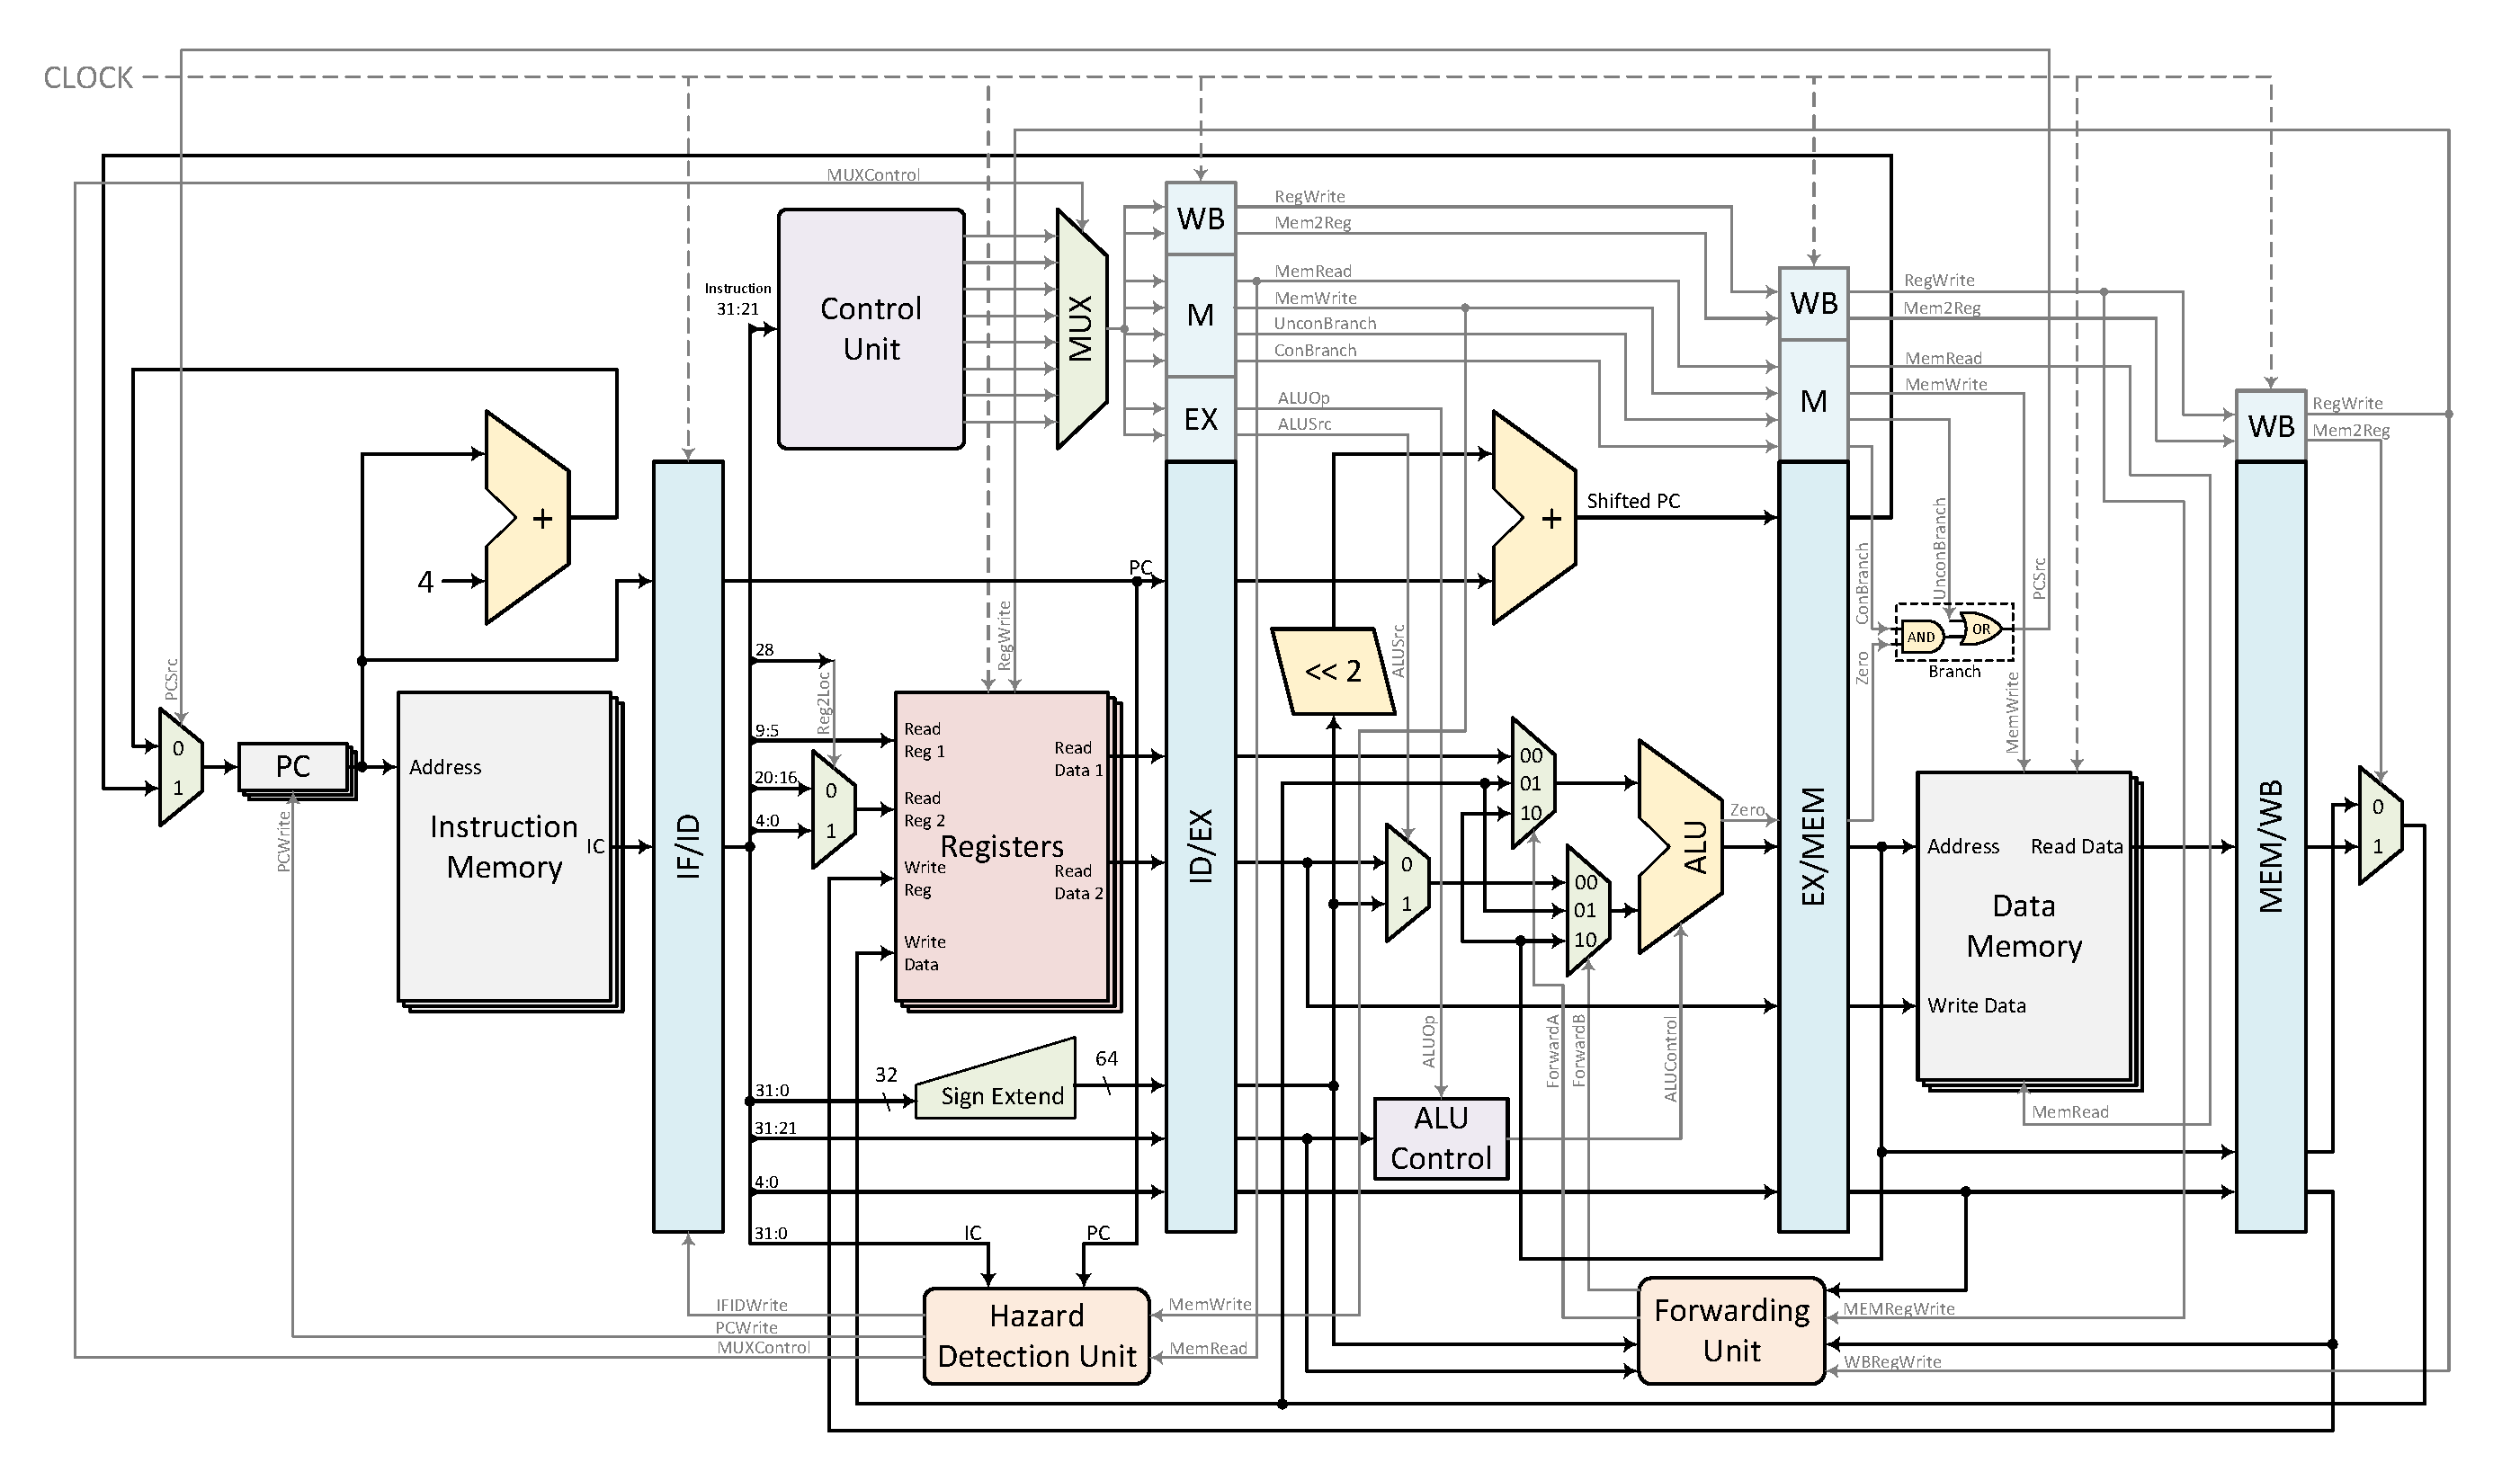
\includegraphics[page=1, width=\linewidth]{ARM_Lite_CPU_full.pdf}
      \caption{ARM Lite CPU design, detailing Fig. 4.63 of \cite{patterson2016computer}.}
      \label{fig:CPU_p1}
    \end{figure}

    There are five periods in this CPU, Instruction Fetch (IF)Instruction Decode (ID), Execute (EX), Memory Access (MEM) and Register write back (WB) which are shown clearly in Fig.~\ref{fig:CPU_p1}, divided by a large register between periods.
    The functions of each components will be elaborated in Chapter~\ref{cha:instructions}.

  \section{Hazard Detection and Forwarding}

    Hazard Detection and Forwarding are both modules that work together to solve the hazard problem.


\chapter{Supported Instructions}\label{cha:instructions}

  \begin{introduction}
    \item R Type Instructions
    \item I Type Instructions
    \item D Type Instructions
    \item B Type Instructions
    \item CB Type Instructions
    \item Data Flow Graphs
  \end{introduction}

  \section{Summary}

    Apart from the instructions already supported by the original project,
    this project adds all I type and CB type instructions and also extend the range of R type instructions like \texttt{LSL}, \texttt{LSR} and \texttt{EOR}.

  \section{R Type}

    \subsection{ADD}

      Example: \texttt{ADD r5, r3, r2} (Add the values of \texttt{r3} and \texttt{r2} then put the result into \texttt{r5})

      \begin{figure}[htbp]
        \centering
        \includegraphics[page=4, width=\linewidth]{ARM_Lite_CPU_full.pdf}
        \caption{Data flows for instructions \texttt{ADD}, \texttt{SUB}, \texttt{AND}, \texttt{ORR}, \texttt{EOR}.}
        \label{fig:CPU_p4}
      \end{figure}

      \begin{itemize}
        \item \texttt{PC} will be incremented by 4 and the shifted \texttt{PC} will be discarded.
        \item Input registers are in \texttt{[20:16]} and \texttt{[9:5]}.
        \item \texttt{ALU MUX} chooses \texttt{0}, i.e. data just read from the registers.
        \item \texttt{ALUControl} will tells \texttt{ALU} to do \texttt{ADD} operation.
        \item No need to write memory but need to write back to registers.
      \end{itemize}

    \subsection{SUB}
      Example: \texttt{SUB r4, r3, r2} (Subtract the values of \texttt{r3} and \texttt{r2} then put the result into \texttt{r4})

      \begin{itemize}
        \item This is similar to \texttt{ADD} instruction except for the operation given by \texttt{ALU Control} to \texttt{ALU}.
      \end{itemize}

    \subsection{AND}

      Example: \texttt{AND r4, r3, r2} (Bit-wise AND the values of \texttt{r3} and \texttt{r2} then put the result into \texttt{r4})

      \begin{itemize}
        \item This is similar to \texttt{ADD} instruction except for the operation given by \texttt{ALU Control} to \texttt{ALU}.
      \end{itemize}

    \subsection{ORR}
      Example: \texttt{ORR r6, r2, r3} (Bit-wise OR the values of \texttt{r2} and \texttt{r3} then put the result into \texttt{r6})

      \begin{itemize}
        \item This is similar to \texttt{ADD} instruction except for the operation given by \texttt{ALU Control} to \texttt{ALU}.
      \end{itemize}

    \subsection{EOR}
      Example: \texttt{EOR r6, r2, r3} (Exclusive OR the values of \texttt{r2} and \texttt{r3} then put the result into \texttt{r6})

      \begin{itemize}
        \item This is similar to \texttt{ADD} instruction except for the operation given by \texttt{ALU Control} to \texttt{ALU}.
      \end{itemize}
    \subsection{LSL}

      Example: \texttt{LSL r6, r2, \#3} (Logical Shift Left the values of \texttt{r2} by 3 then put the result into \texttt{r6})

      \begin{figure}[htbp]
        \centering
        \includegraphics[page=5, width=\linewidth]{ARM_Lite_CPU_full.pdf}
        \caption{Data flows for instructions \texttt{ADDI}, \texttt{SUBI}, \texttt{ANDI}, \texttt{ORRI}, \texttt{EORI}, \texttt{LSL}, \texttt{LSR}.}
        \label{fig:CPU_p5}
      \end{figure}

      \begin{itemize}
        \item \texttt{PC} will be incremented by 4 and the shifted \texttt{PC} will be discarded.
        \item Input register is in \texttt{[9:5]}.
        \item \texttt{ALU MUX} chooses \texttt{1}, i.e. data coming from \texttt{Sign Extend}, the \texttt{shamt} part in the machine code.
        \item \texttt{ALUControl} will tells \texttt{ALU} to do \texttt{LSL} operation.
        \item No need to write memory but need to write back to registers.
      \end{itemize}
      
    \subsection{LSR}

      Example: \texttt{LSR r6, r2, \#3} (Logical Shift Right the values of \texttt{r2} by 3 then put the result into \texttt{r6})

      \begin{itemize}
        \item This is similar to \texttt{LSL} instruction except for the operation given by \texttt{ALU Control} to \texttt{ALU}.
      \end{itemize}

  \section{I Type}

    \subsection{ADDI}

      Example: \texttt{ADDI r5, r3, \#2} (Add the values of \texttt{r3} and immediate 2 then put the result into \texttt{r5})

      \begin{itemize}
        \item Different from instruction \texttt{ADD}, the immediate comes from the \texttt{Sign Extend} and the \texttt{ALU MUX} chooses the immediate out value.
      \end{itemize}
      

    \subsection{SUBI}

      Example: \texttt{SUBI r4, r3, \#2} (Subtract the values of \texttt{r3} with immediate 2 then put the result into \texttt{r4})

      \begin{itemize}
        \item This is similar to \texttt{ADDI} instruction except for the operation given by \texttt{ALU Control} to \texttt{ALU}.
      \end{itemize}

    \subsection{ANDI}

      Example: \texttt{ANDI r4, r3, \#2} (Bit-wise AND the values of \texttt{r3} and 2 then put the result into \texttt{r4})

      \begin{itemize}
        \item This is similar to \texttt{ADDI} instruction except for the operation given by \texttt{ALU Control} to \texttt{ALU}.
      \end{itemize}

    \subsection{ORRI}

      Example: \texttt{ORRI r6, r2, \#3} (Bit-wise OR the values of \texttt{r2} and 3 then put the result into \texttt{r6})

      \begin{itemize}
        \item This is similar to \texttt{ADDI} instruction except for the operation given by \texttt{ALU Control} to \texttt{ALU}.
      \end{itemize}


    \subsection{EORI}

      Example: \texttt{EORI r6, r2, \#3} (Exclusive OR the values of \texttt{r2} and 3 then put the result into \texttt{r6})

      \begin{itemize}
        \item This is similar to \texttt{ADDI} instruction except for the operation given by \texttt{ALU Control} to \texttt{ALU}.
      \end{itemize}

  \section{D Type}

    \subsection{LDUR}

      Example 1: \texttt{LDUR r2, [r10]} (Retrieve the value in memory at location \texttt{r10} and put that value into register \texttt{r2})

      Example 2: \texttt{LDUR r3, [r10, \#1]} (Retrieve the value in memory at the location \texttt{r10} + immediate (1) and put that value into register \texttt{r3})

      \begin{figure}[htbp]
        \centering
        \includegraphics[page=2, width=\linewidth]{ARM_Lite_CPU_full.pdf}
        \caption{Data flow for instruction \texttt{LDUR}.}
        \label{fig:CPU_p2}
      \end{figure}

      \begin{itemize}
        \item \texttt{PC} will be incremented by 4 and the shifted \texttt{PC} will be discarded.
        \item Input register is in \texttt{[9:5]}.
        \item \texttt{ALU MUX} chooses \texttt{1}, i.e. data coming from \texttt{Sign Extend}, the addition to register value. Then the result of them will be the data to write back.
        \item \texttt{ALUControl} will tells \texttt{ALU} to do \texttt{ADD} operation.
        \item No need to write memory but need to write back to registers.
        \item It should be noticed that not until the end of period \texttt{MEM} the result is not given out. This is different from instructions of R or I types where the calculation result comes immediately after \texttt{ALU}, i.e. the period of \texttt{EX}.
      \end{itemize}

    \subsection{STUR}

      Example 1: \texttt{STUR r1, [r9]} (Store the value of \texttt{r1} into memory at the location \texttt{r9})

      Example 2: \texttt{STUR r4, [r7, \#1]} (Store the value of \texttt{r4} into memory at the location \texttt{r7} + immediate (1))

      \begin{figure}[htbp]
        \centering
        \includegraphics[page=3, width=\linewidth]{ARM_Lite_CPU_full.pdf}
        \caption{Data flow for instruction \texttt{STUR}.}
        \label{fig:CPU_p3}
      \end{figure}

      \begin{itemize}
        \item \texttt{PC} will be incremented by 4 and the shifted \texttt{PC} will be discarded.
        \item Input register is in \texttt{[9:5]}.
        \item \texttt{ALU MUX} chooses \texttt{1}, i.e. data coming from \texttt{Sign Extend}, the addition to register value. Then the result of them will be the data to write back.
        \item \texttt{ALUControl} will tells \texttt{ALU} to do \texttt{ADD} operation.
      \end{itemize}

  \section{B Type}
    \subsection{B}

      \begin{figure}[htbp]
        \centering
        \includegraphics[page=6, width=\linewidth]{ARM_Lite_CPU_full.pdf}
        \caption{Data flow for instruction \texttt{B}.}
        \label{fig:CPU_p6}
      \end{figure}

      Example: \texttt{B \#2} (Jump instruction with 2)

      \begin{itemize}
        \item With the Unconditional Jump signal, the \texttt{PC} is set to the shifted \texttt{PC}.
      \end{itemize}

  \section{CB Type}
    \subsection{CBZ}

      Example: \texttt{CBZ r1, \#2} (If the value of \texttt{r1} is zero then jump to instruction 2, otherwise, continue executing \texttt{PC++})

      \begin{figure}[htbp]
        \centering
        \includegraphics[page=7, width=\linewidth]{ARM_Lite_CPU_full.pdf}
        \caption{Data flows for instructions \texttt{CBZ}, \texttt{CBNZ}.}
        \label{fig:CPU_p7}
      \end{figure}

      \begin{itemize}
        \item The Conditional Branch is set to \texttt{1}.
        \item The most important thing here is the \texttt{Zero} flag of \texttt{ALU}. The operation of \texttt{ALU} is takes the value of \texttt{[4:0]} directly. Therefore, the result of the \texttt{Branch} module generates the \texttt{PCSrc} signal that decides whether \texttt{PC} to jump.
      \end{itemize}

    \subsection{CBNZ}

      Example: \texttt{CBNZ r1, \#2} (If the value of \texttt{r1} is not zero then jump to instruction 2, otherwise, continue executing \texttt{PC++})

      \begin{itemize}
        \item The Conditional Branch is set to \texttt{1}.
        \item The most important thing here is the \texttt{Zero} flag of \texttt{ALU}. The operation of \texttt{ALU} is takes the logic \textsc{Not} of \texttt{[4:0]}. Therefore, the result of the \texttt{Branch} module generates the \texttt{PCSrc} signal that decides whether \texttt{PC} to jump.
      \end{itemize}

\chapter{Simulation Examples}

  \begin{introduction}
    \item Behavioral Simulation
    \item Simulation Waveforms
    \item Instructions Analysis
  \end{introduction}

  \section{Example 1}

    \begin{lstlisting}[language={[x86masm]Assembler}, columns=fixed, morekeywords={LDUR,ADDI,ANDI,SUBI,B}]
LDUR x0, [x2, #3] ; f8403040
ADDI x5, x9, 7    ; 91001d25
ANDI x3, x3, 3    ; 92000c63
SUBI x6, x6, 3    ; d1000cc6
LSL  x7, 1        ; d36004e7
B    -3           ; 17fffffd
    \end{lstlisting}

    \begin{figure}[htbp]
      \centering
      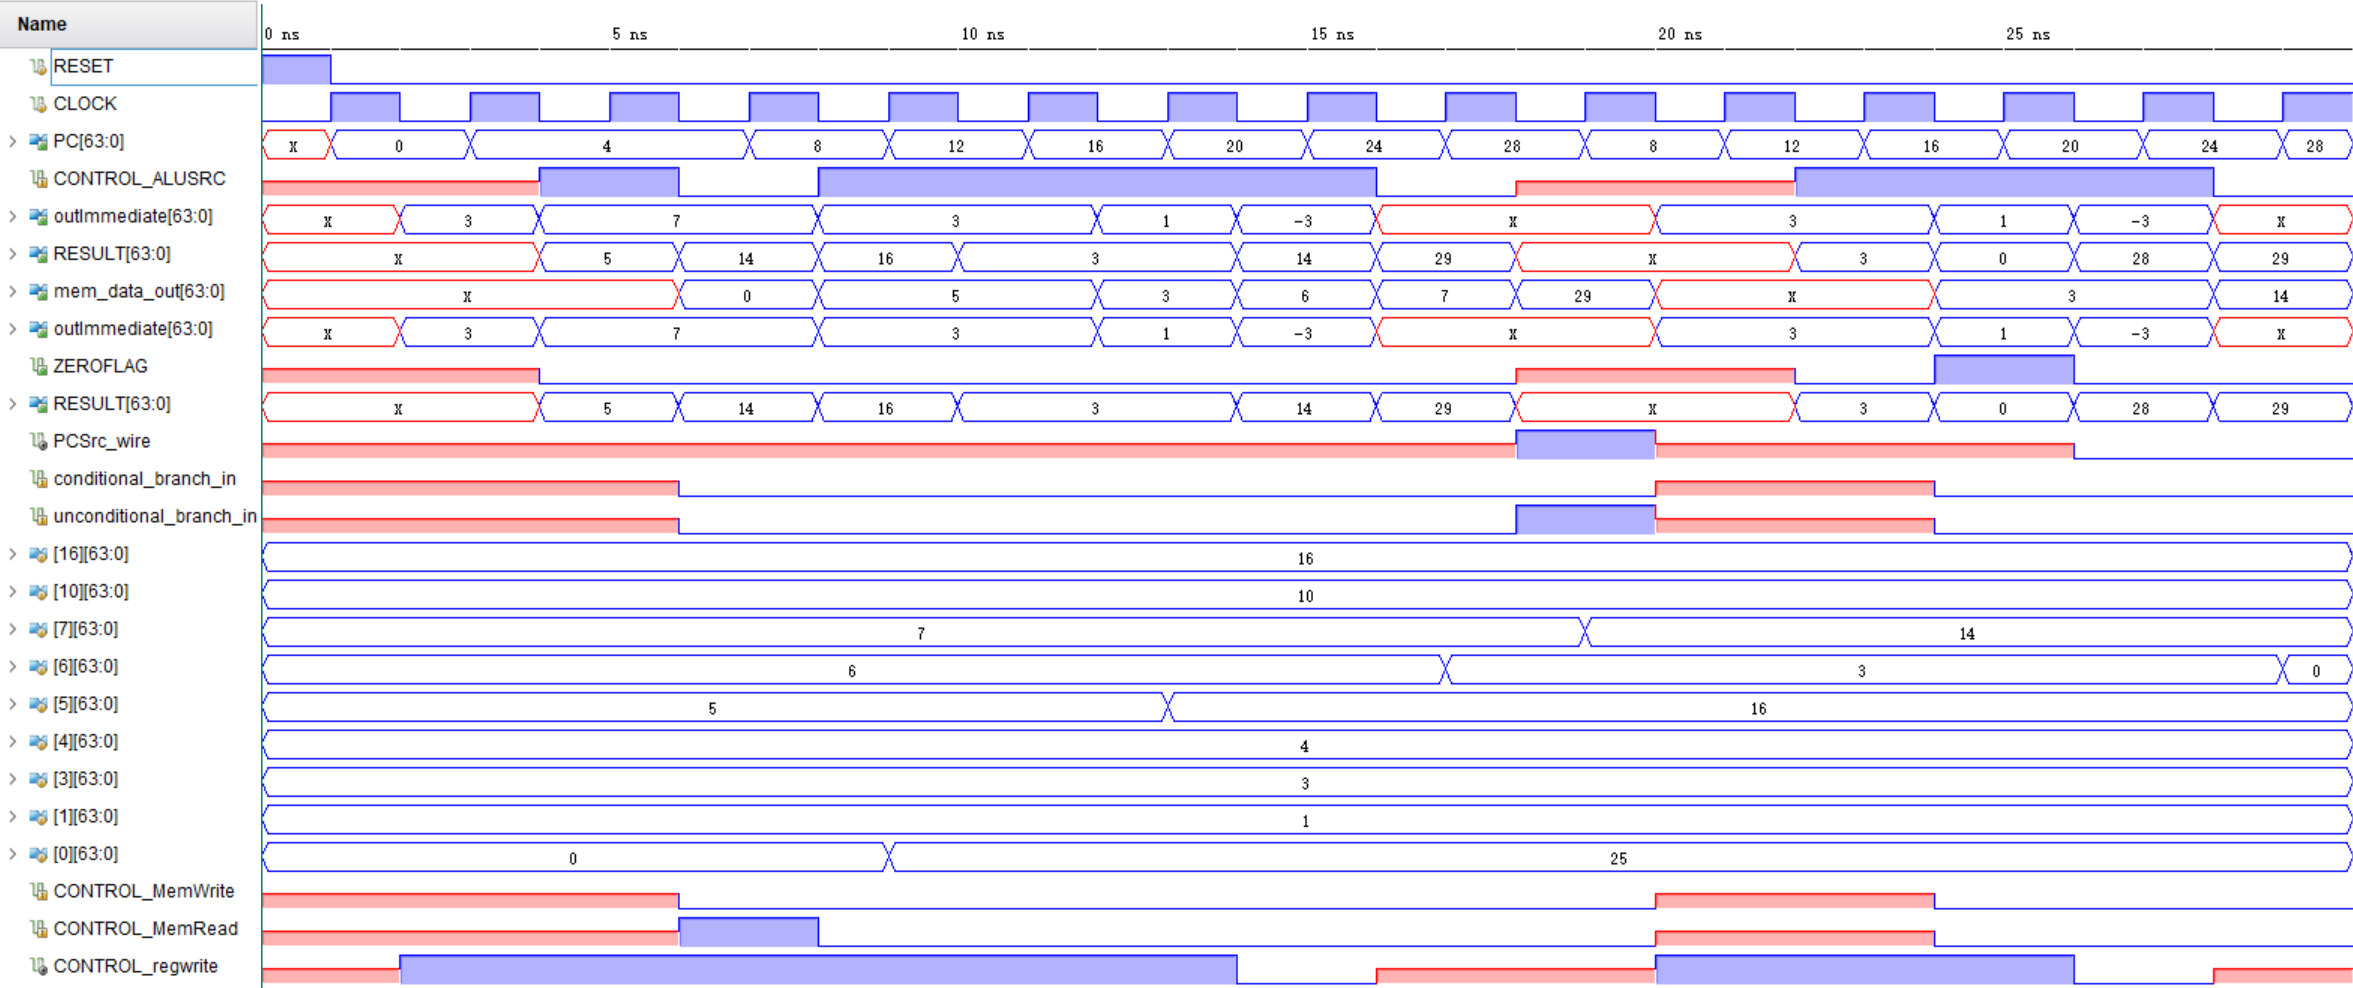
\includegraphics[width=\linewidth]{wave/Example 1.png}
      \caption{Simulation Waveforms for Example 1}
      \label{fig:sim_1}
    \end{figure}

    With the IF, ID, EX, MEM and WB stages of a pipelined CPU, each instruction is executed at the positive edge of the clock signal.
    Therefore, there will be five occurrences of the positive edges during one cycle of an instruction.
    
    In example 1, six instructions are used.

    During the \texttt{LDUR} instruction, \texttt{PC=0}.
    When \texttt{PC=4}, \texttt{x2} is read from the registers.
    This value is then added with the immediate value from \texttt{Sign Extend}.
    (Because of the hazard detection, one \texttt{NOP} is added automatically.)
    From the third positive edge, \texttt{ALU} executes the addition  of \texttt{x2} and \texttt{3}. In the fourth positive edge, the value of \texttt{RAM[5]} is read out (We can find the \texttt{MemRead} control signal during 6-8 ns).
    From the fifth positive edge, \texttt{x1} and \texttt{RAM[5]} is returned to the registers and then \texttt{x1=RAM[5]}.
    Because of \texttt{NOP}, \texttt{ADDI} instructions come from the the third positive edge and write back at the 8th positive edge.
    When dealing with immediate values, \texttt{ALUSrc} signal is set to 1.

    It is similar for \texttt{ANDI}, \texttt{SUBI}, \texttt{LSL} commands, and the changes of values in registers can also be observed.

    Because the jump by instruction \texttt{B} occurs in the fourth clock period, \texttt{PC} jumps from 28 to 8, forming a loop.
    When the jump is required, \texttt{PCSrc} is set to 1.

  \section{Example 2}

      \begin{lstlisting}[language={[x86masm]Assembler}, columns=fixed, morekeywords={LDUR,LSR,EOR,CBZ,ORRI,EORI,STUR}]
LDUR x0 , [x2, #3] ; f8403040
LSR  x16, #1       ; d3400610
EOR  x1 , x2 , x0  ; ca000041
CBZ  x31, #8       ; b400011f
ORRI x4 , x5 , 7   ; b2001ca4
EORI x10, x11, #11 ; d2002d6a
; SKIP THREE LINES ;
ORRI x4 , x5 , 7   ; b2001ca4
EORI x10, x11, #11 ; d2002d6a
STUR x11, [x5, #6] ; f80060ab
    \end{lstlisting}

    \begin{figure}[htbp]
      \centering
      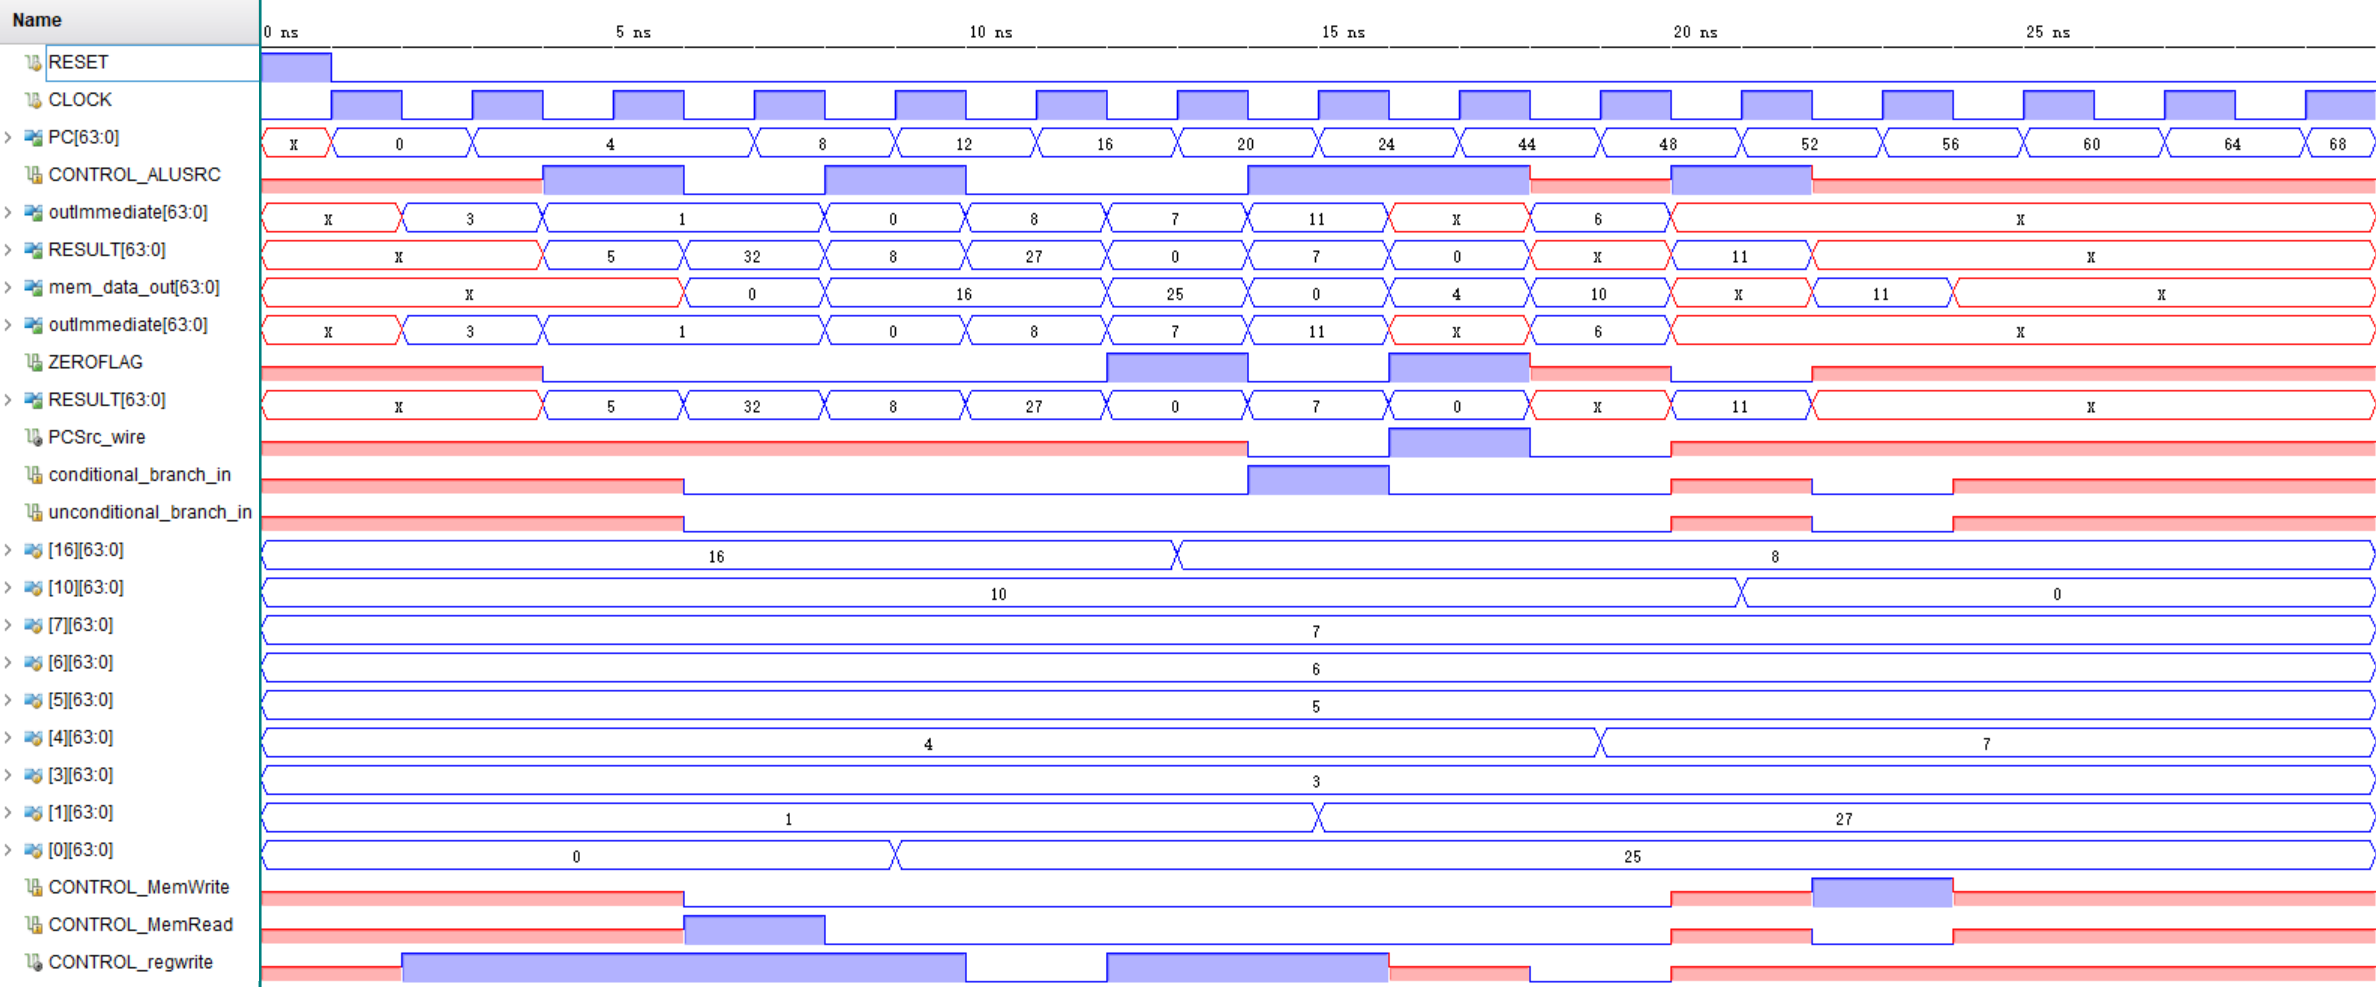
\includegraphics[width=\linewidth]{wave/Example 2.png}
      \caption{Simulation Waveforms for Example 2}
      \label{fig:sim_2}
    \end{figure}

    Here we elaborate on the conditional branch \texttt{CBZ} instruction.
    First the \texttt{ZERO} flag is 1 in 12-14 ns and then conditional branch signal is 1 in 14-16 ns.
    Therefore, the branch will get the result 1 in 16-18 ns.
    In the next clock period, the \texttt{PCSrc} will be set as 1 and then the conditional jump succeeds.

\chapter{Known Issues}

    \section{CPU Project}

      \begin{itemize}
        \item Hazard Detection and Forwarding is naive and cannot tell exactly tell where forwarding or \texttt{NOP} is needed.
        \item Control hazard can not be solved so far and can lead to fatal error in simulation.
      \end{itemize}

    \section{Compiler}

      This work is still under progress and should be finished in the following weeks.


\chapter{Version History}
We revised our project now and then. This section shows the version story of ARM Lite. We have 37 commits and 2 releases on GitHub.


\datechange{2022/01/07}{release of v2.0}

\begin{change}
  \item Solve the bug with instructions \texttt{CBZ} and \texttt{CBNZ}.
  \item Add Simulation Test.
\end{change}

\datechange{2021/12/24}{release of v1.1}

\begin{change}
  \item Add instructions.
\end{change}

\datechange{2021/12/23}{release of v1.0}

\begin{change}
  \item Work based on \href{https://github.com/nxbyte/ARM-LEGv8}{ARM-LEGv8} (pipelined with hazard detection and forwarding) is implemented on Xilinx Vivado 2017.4 both on Ubuntu and Windows.
  \item Create the Visio Drawing for the CPU architecture.
\end{change}

\nocite{en2,en3}
\clearpage
\phantomsection % let the href jump to the right page
\addcontentsline{toc}{chapter}{Bibliography}
\printbibliography

\appendix
% \renewcommand\chaptername{\eappendix \thechapter}

\chapter{Future Work}

Issues listed will be dealt with and a better documentation will be done together with the online documentation.

Moreover, an essay about the design of ARM Lite CPU will also be on the agenda.

\begin{figure}[htbp]
  \centering
  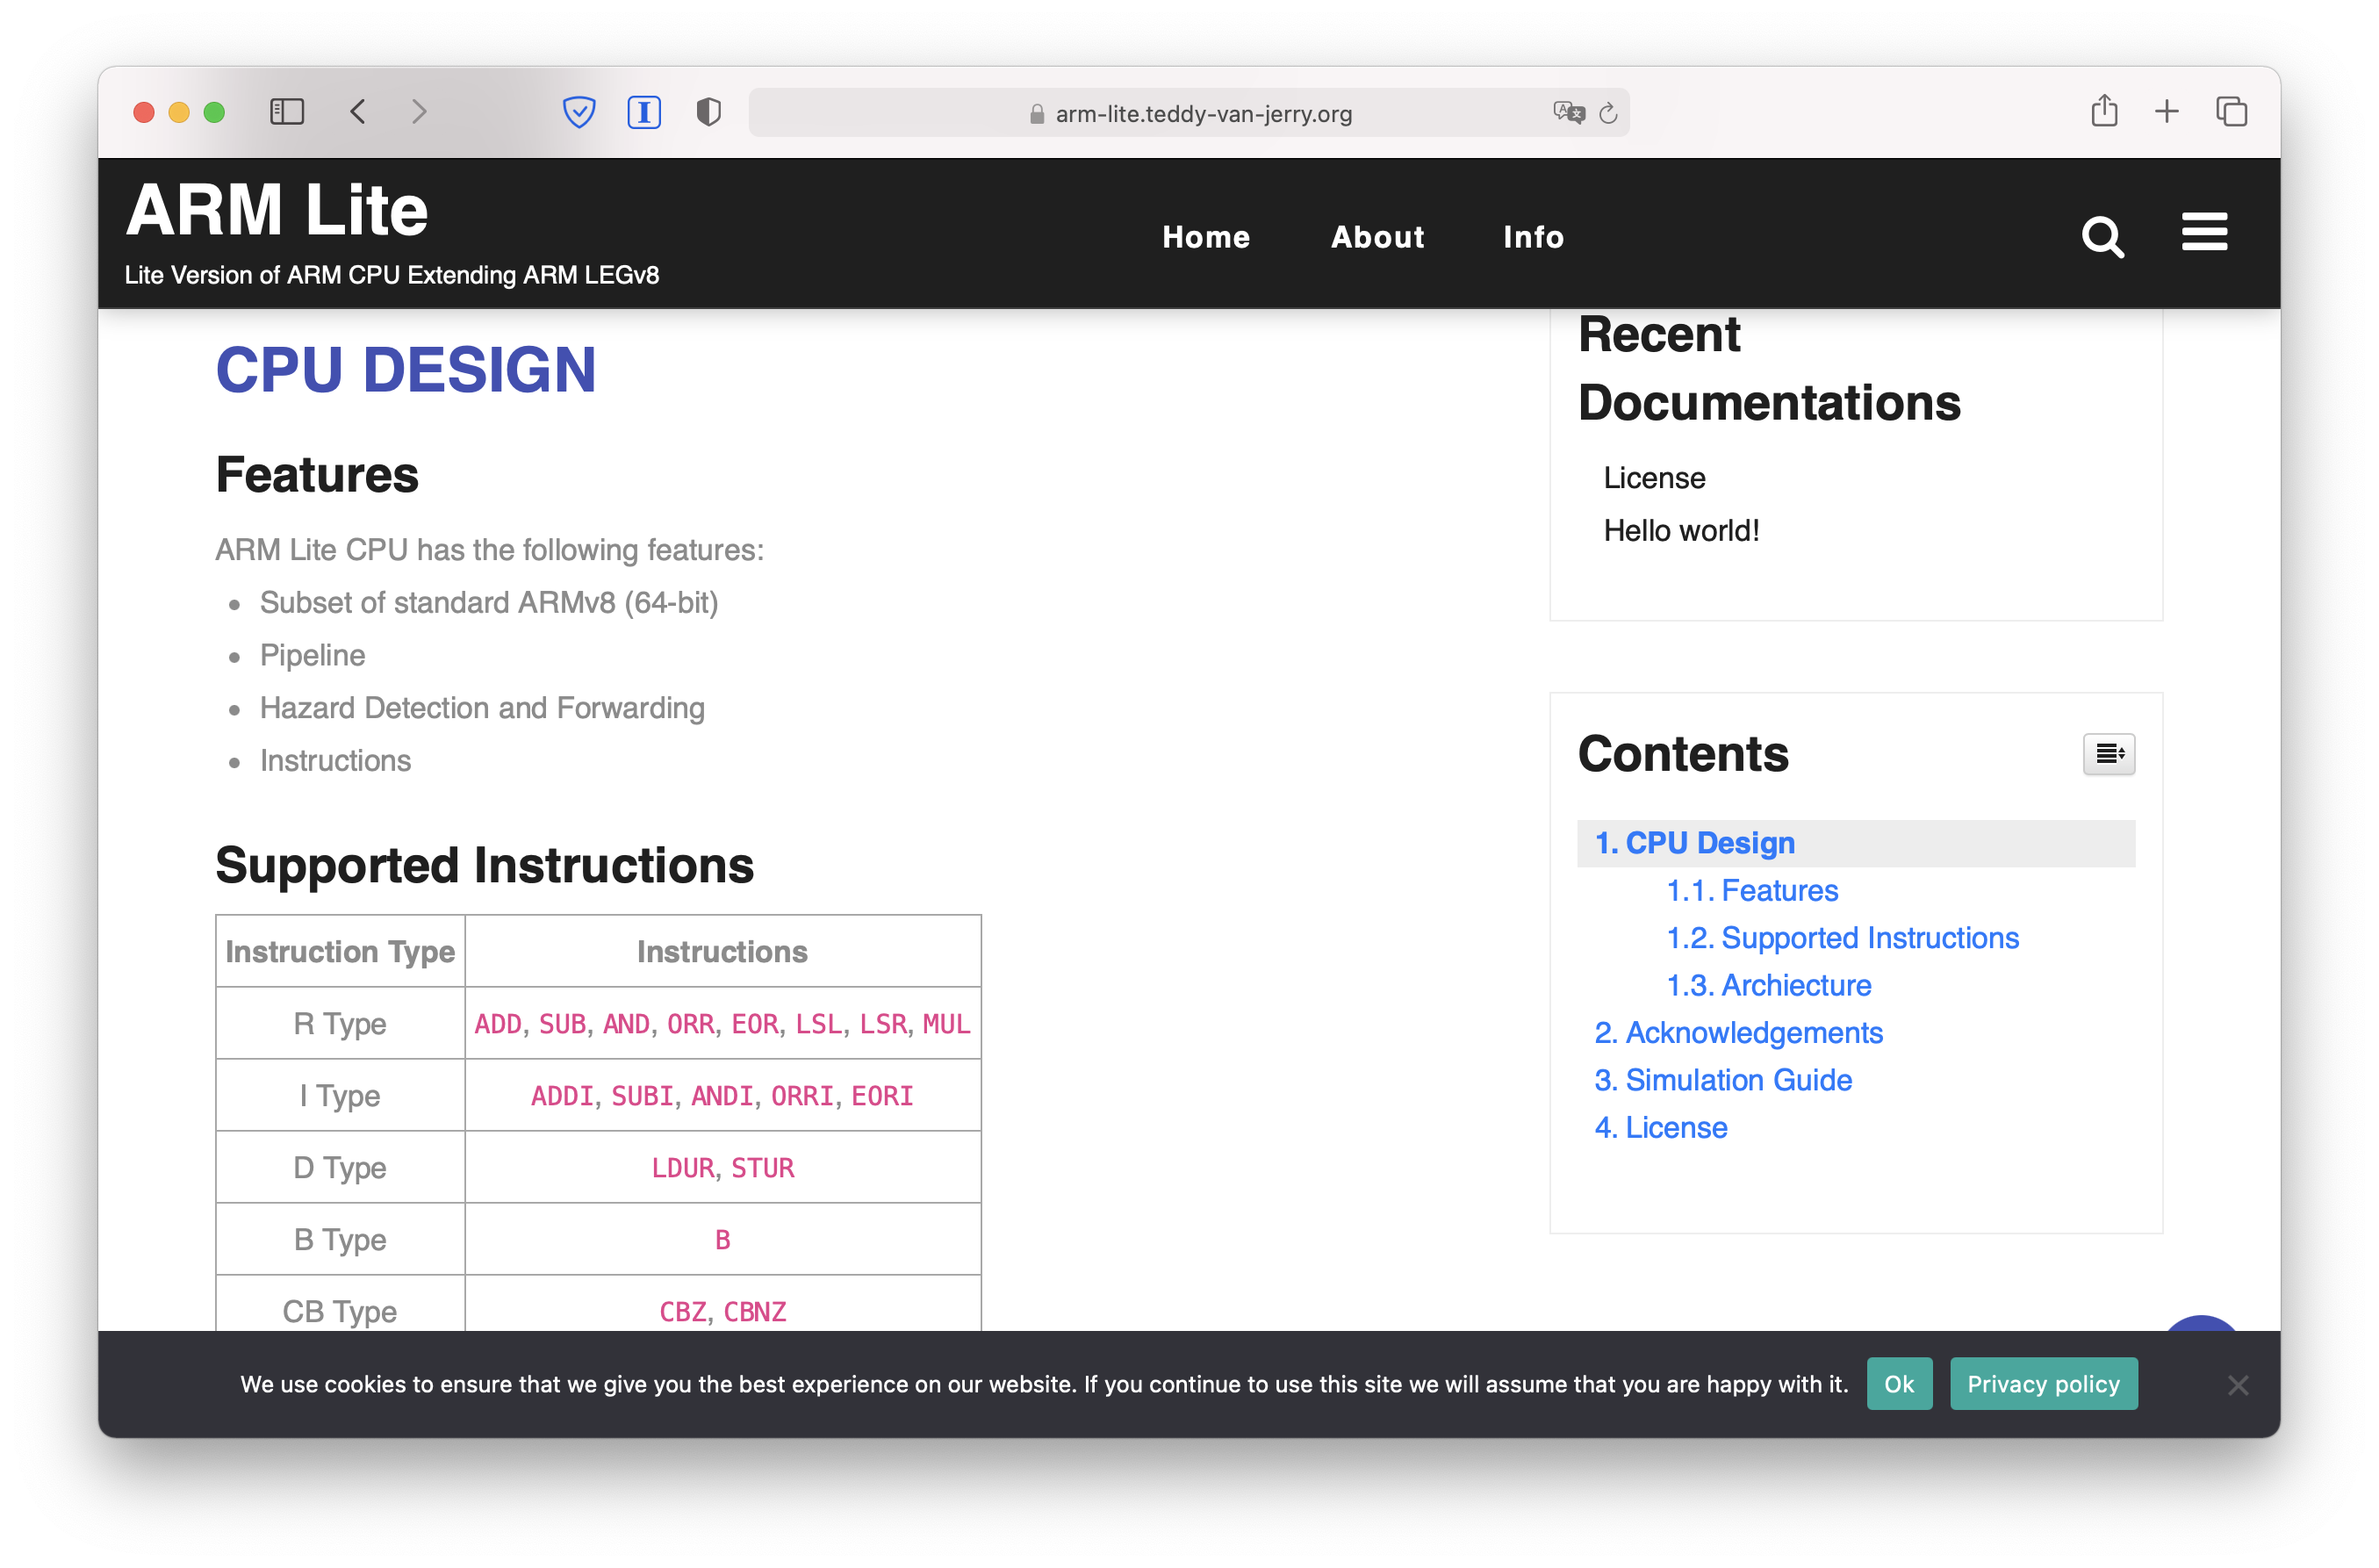
\includegraphics[width=\linewidth]{image/website.png}
  \caption{ARM Lite website.}
\end{figure}



\end{document}